\documentclass[a4paper]{article}

\usepackage{caption}
\usepackage{subcaption}
% accetta caratteri complicati tipo vocali accentate
\usepackage[T1]{fontenc}
\usepackage[utf8]{inputenc}


%collegamenti ipertestuali
\usepackage{hyperref}

%tabelle
\usepackage{booktabs}
\captionsetup[figure]{font=scriptsize}

%grafici
\usepackage{graphicx}

%matematica
\usepackage{mathtools}
\usepackage{amsmath}

%stile di pagine
\pagestyle{plain} %headings?

%Notes
\usepackage{fancyhdr}
\usepackage{wrapfig}% layout
\usepackage[export]{adjustbox}
\usepackage[colorinlistoftodos]{todonotes}						% pour faire des notes	
\usepackage[toc,page]{appendix}


\usepackage{enumerate}
\usepackage[english]{babel}
\usepackage{lmodern}
\usepackage{amsfonts,amssymb}
\usepackage[a4paper, margin=1in]{geometry}
\usepackage[parfill]{parskip}
\usepackage{epstopdf}
\usepackage{color}
\usepackage[tt]{titlepic}
\usepackage{fancyhdr}
\usepackage{enumerate}
\usepackage{lastpage}
%\usepackage{subfigure}
\usepackage{bm}
\usepackage{verbatim}
\usepackage{listings}
\usepackage{tasks}
\usepackage{float}
%\pagenumbering{gobble}



\begin{document}

\newcommand*\xbar[1]{%
  \hbox{%
    \vbox{%
      \hrule height 0.5pt % The actual bar
      \kern0.5ex%         % Distance between bar and symbol
      \hbox{%
        \kern-0.1em%      % Shortening on the left side
        \ensuremath{#1}%
        \kern-0.5em%      % Shortening on the right side
      }%
    }%
  }%
} 

%\interfootnotelinepenalty=10000
\begin{titlepage}
	\vspace{50mm}
	\begin{center}
		
\includegraphics[width=5cm]{Figures/EPFL_LOG.pdf}\\
		\vspace{2cm}
		%{\large{\bf }}\\
		\vspace{5mm}
		{\LARGE{\bf Financial Big Data Project}}\\
		\vspace{3mm}
		{\large{\bf Algorithmic Trading on FX High Frequency Data}}\\
		%\vspace{19mm} {\large{\bf }}
	\end{center}
	\vspace{60mm}
	\par
	\noindent
	%\begin{center}

			{\large{\bf Realized by: \\
            
            		\vspace{10pt}
                    
					ALESSANDRO DANIELE FORLONI\\
					MATTEO PIETROBON\\
				}}
	%\end{center}
	
	\vspace{10pt}
	\begin{center}
		{\large{\bf Academic Year\\
				2017/2018 }}
	\end{center}
\end{titlepage}

\newpage
\tableofcontents

\newpage

%COMMENTS LIKE THIS
%\todo[inline, color=red!50]{Some Comment}

%IF WE NEED TO CITE SOMETHING USE: \cite{example}.

\section{Abstract}

During the semester we learned sophisticated ways to extract information from our data and clever methods to deal with it when it is too abundant. In this project we wanted to show our skills on both those aspects, keeping in mind the important trade-off between the amount of data that we are handling and the complexity of the operations that we are performing on it.\\
In order to do that, we decided that our best option was to implement two different strategies. The first is quite basic in its principle, but it was executed on the overwhelming amount of data that we collected. The other strategy allowed us to showcase a deeper financial intuition, but, due to the higher computational burden, we only applied it to the \todo{applied where?}


\section{Introduction}

We tried to structure our report in a narrative way, presenting both the issues that we faced and the solutions that we applied. As mentioned in the abstract, we developed two different strategies for our project. Both strategies use the same data, high-frequency FX data. Their rationale and results are quite independent and will, therefore, be presented separately.\\
All our strategies are built through adapted processes, i.e. we only use past information to make decisions.\\ 


\section{Data Description}

We decided to use FX high-frequency data because of its abundance and because of our personal interest in this field. We focused on 5 currency pairs:
\begin{itemize}
\item EUR / USD
\item EUR / CHF
\item EUR / GBP
\item EUR / JPY
\item EUR / AUD
\end{itemize}
The time series start on January $1^{\text{st}}$ 2003 and end on December $31^{\text{st}}$ 2016 and it provides Bid and Ask prices for each pair. The data was stored tick-by-tick and grouped in monthly \emph{csv} files, whose size was obviously changing month-by-month.\\
We downloaded the same data for the first 11 months of 2017 and used it to test out-of-sample our strategies.


\subsection{Downloading the data} 

We downloaded the data from this \href{http://www.histdata.com/download-free-forex-historical-data/?/ascii/tick-data-quotes}{Website}. It provides free high-frequency FX data for several currency pairs. We chose the longest series that had EUR as a common reference.\\
We had to download a different file for every currency pair, year and month (5 x 14 x 12 = 840, not even counting the 2017 files). Therefore, we decided to automate the process. However, we could not just access the files through an \emph{url}, the 'download' link was a javascript on the web page so we had to use the \emph{Selenium} package to click on it. We ran this script overnight and stored the data locally. \\
We finally had 895 files, with a total size of 25.1 Gb. The whole process took around 5 hours.

\subsection{Data wrangling} 

We decided to keep our series separate because our strategies were not exploiting cross-currency relations. We aggregated the files by year, but kept the separation into months within them thanks to the structure of \emph{hdf} files.\\
We noticed that the original files were composed of a column with the timestamp, the Bid price, the Ask price and a column of zeros. We removed the last column and transformed the timestamp in a datetime object, that is easier to handle in Python.\\
We checked a portion of the data for the presence of \emph{NaN}s but we could not find any, nonetheless we included a command to drop all the rows which might have contained them. We also checked for the presence of outliers and we found around 10 of them for GBP, CHF and JPY in 2004. They might have been flash crashes but we could find no reference to them in the news and decided to drop those entries. The data after 2004 seems to be much more reliable.\\
Another issue that we found was that the order of the Bid and the Ask column was reversed in June 2009. This was quite easy to solve, but harder to spot because it was not mentioned in the website that we used to download the data.\\
Finally, we have no data during the weekends.\\
We stored the data in \emph{hdf} format, in this way the datetime object was preserved. Finally we had 75 files with a total size of around 17.5 Gb. The whole process took around 1 hour.

\subsection{Descriptive Statistics} 

In Figure \ref{fig:1}, \ref{fig:2}, \ref{fig:3}, \ref{fig:4}, \ref{fig:5} and \ref{fig:6} we report some of the descriptive statistics for the resulting data. We can see that the amount of transactions per year is steadily increasing, reflecting the digitalization of the process. Moreover, we can see that the price process is relatively stable and the drift is close to zero, this is typical of FX data.\\
Please note that we have not examined the testing data.

\begin{figure}
	\centering
	\begin{minipage}{.5\textwidth}
		\centering
		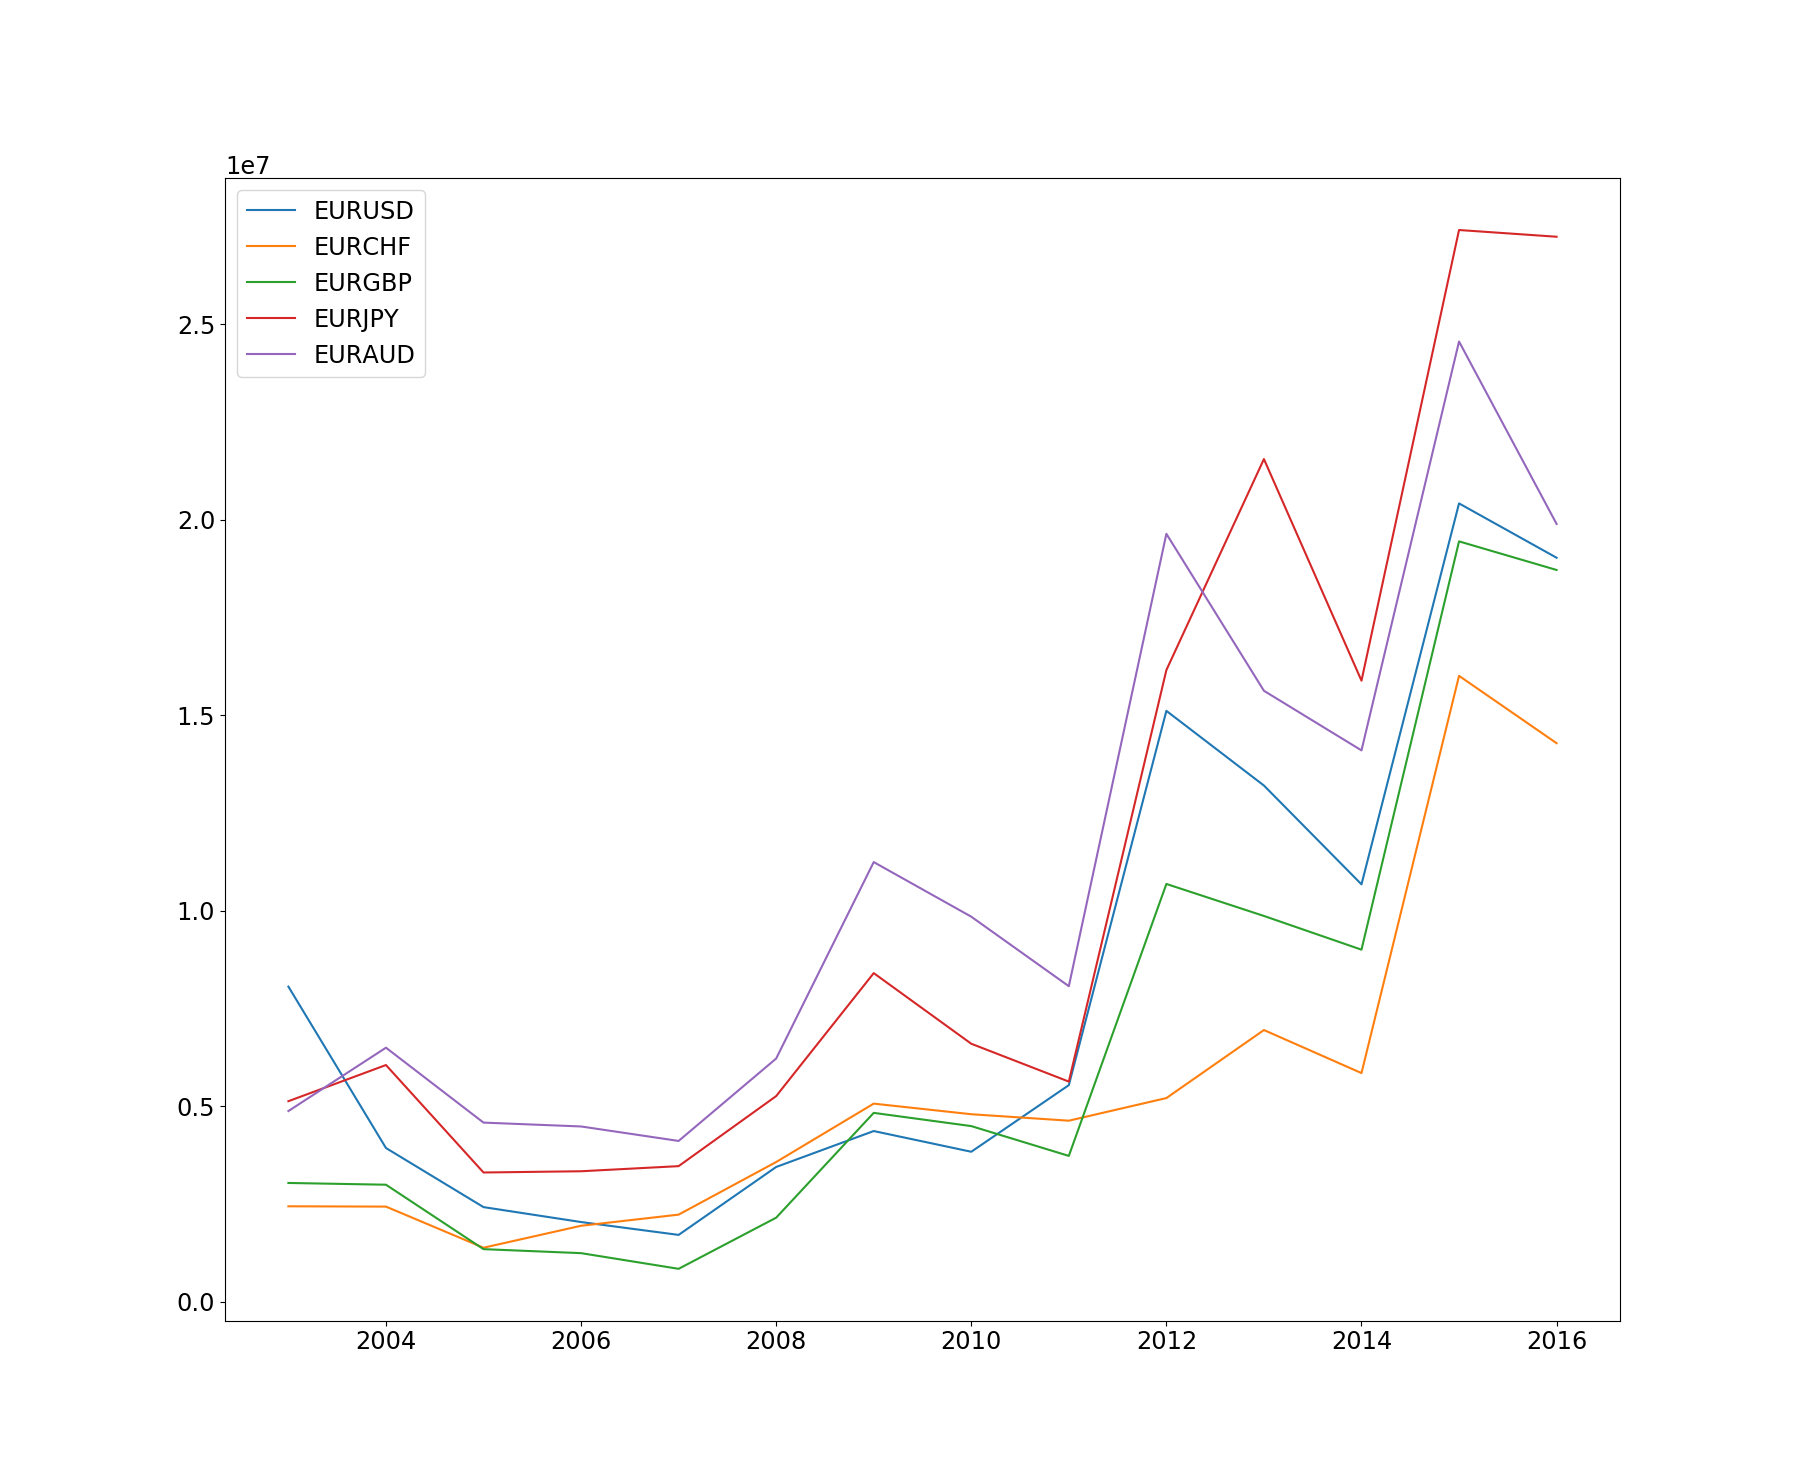
\includegraphics[width=\linewidth]{Figures/counts}
		\captionof{figure}{Data Entries by Currency each Year}
		\label{fig:1}
	\end{minipage}%
	\begin{minipage}{.5\textwidth}
		\centering
		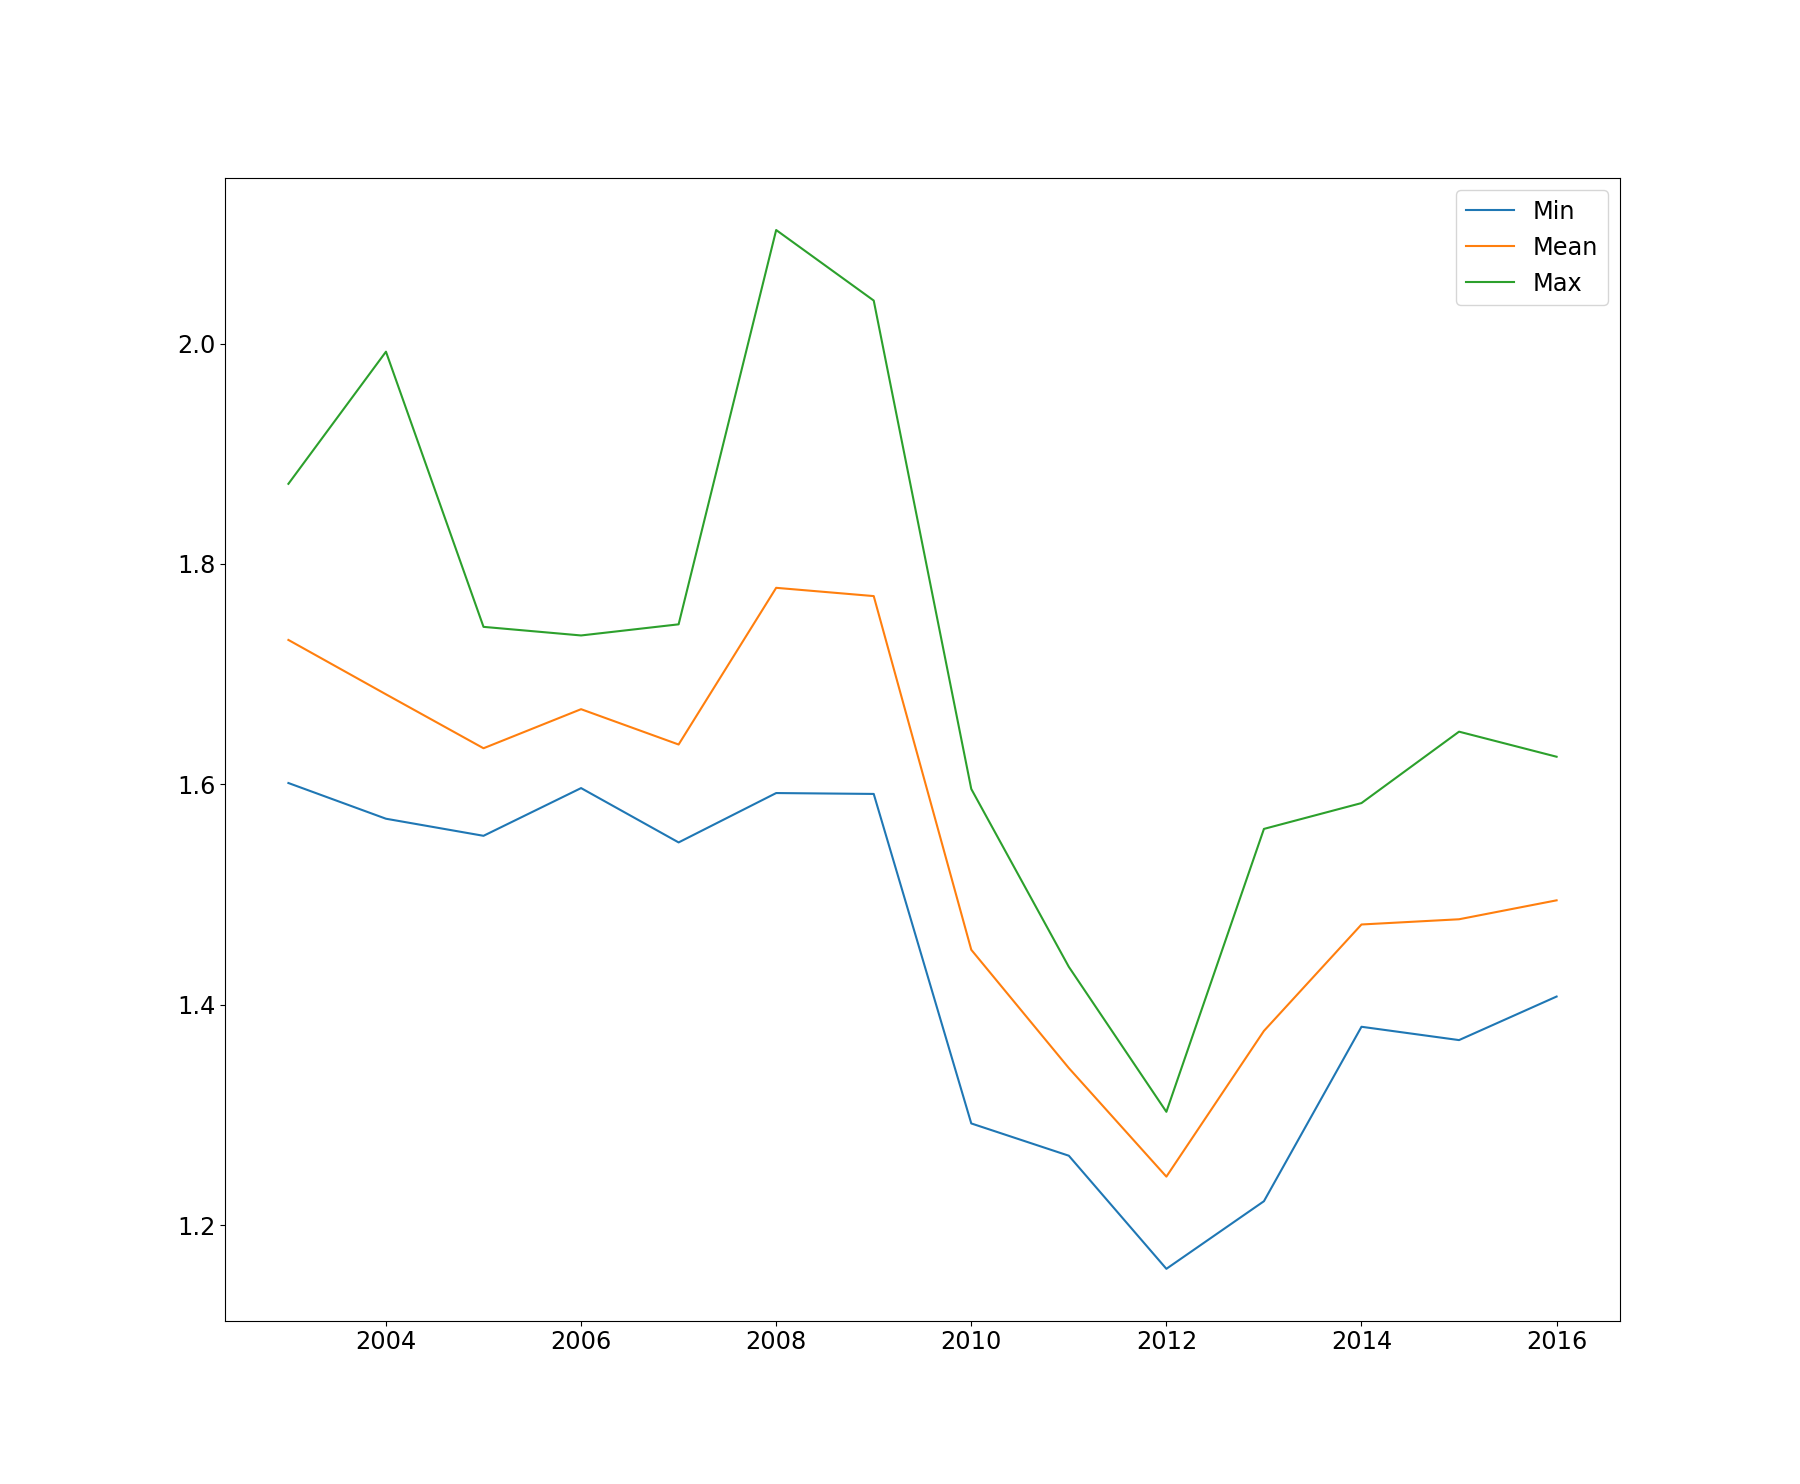
\includegraphics[width=\linewidth]{Figures/stats_aud}
		\captionof{figure}{Min, Mean and Max of EURAUD each year}
		\label{fig:2}
	\end{minipage}
	\begin{minipage}{.5\textwidth}
	\centering
	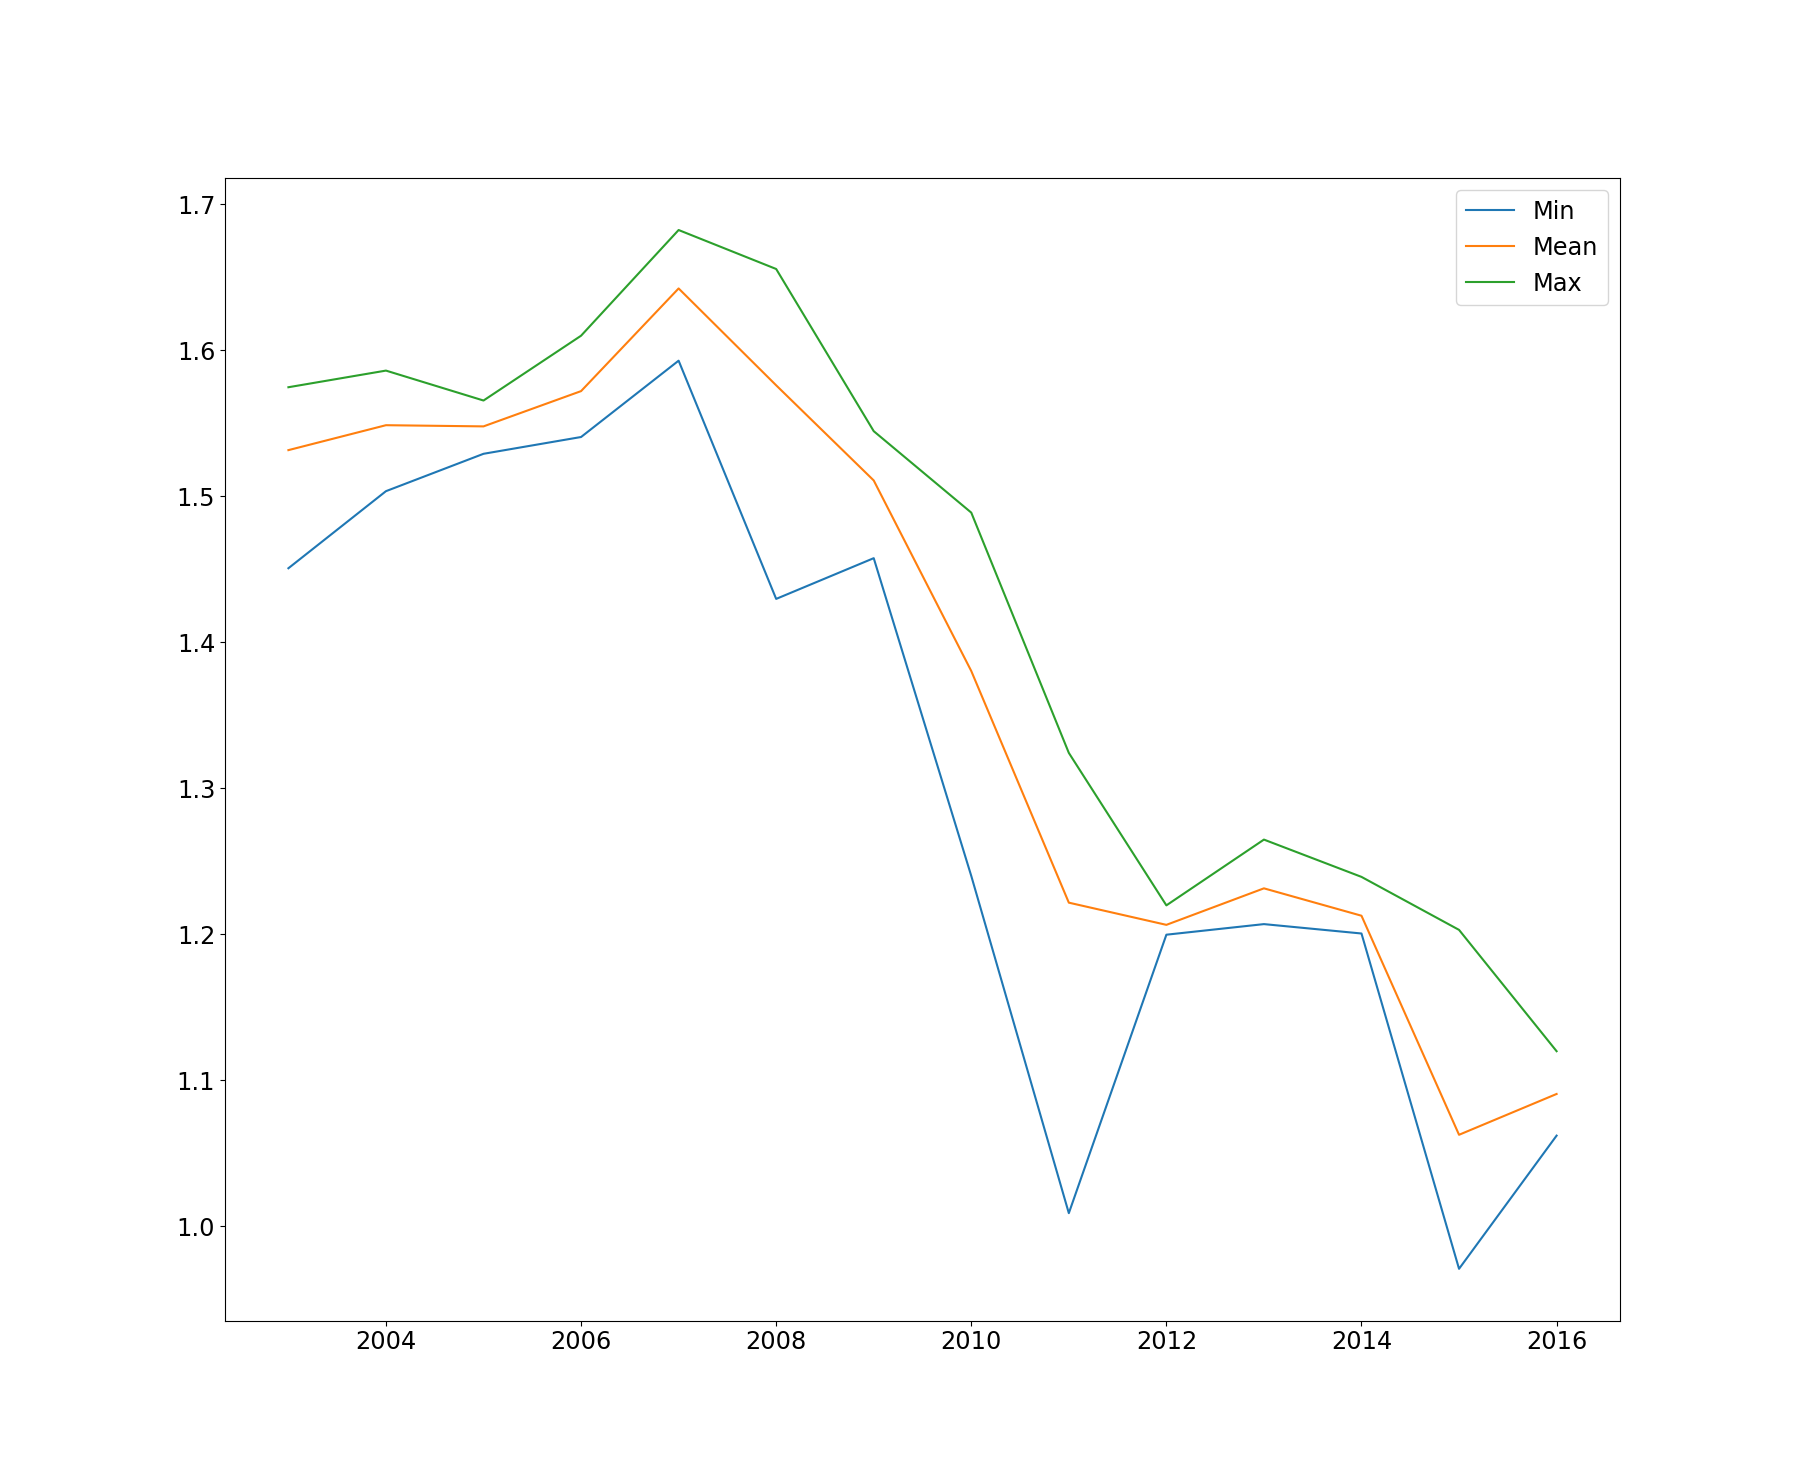
\includegraphics[width=\linewidth]{Figures/stats_chf}
	\captionof{figure}{Min, Mean and Max of EURCHF each year}
	\label{fig:3}
	\end{minipage}%
	\begin{minipage}{.5\textwidth}
	\centering
	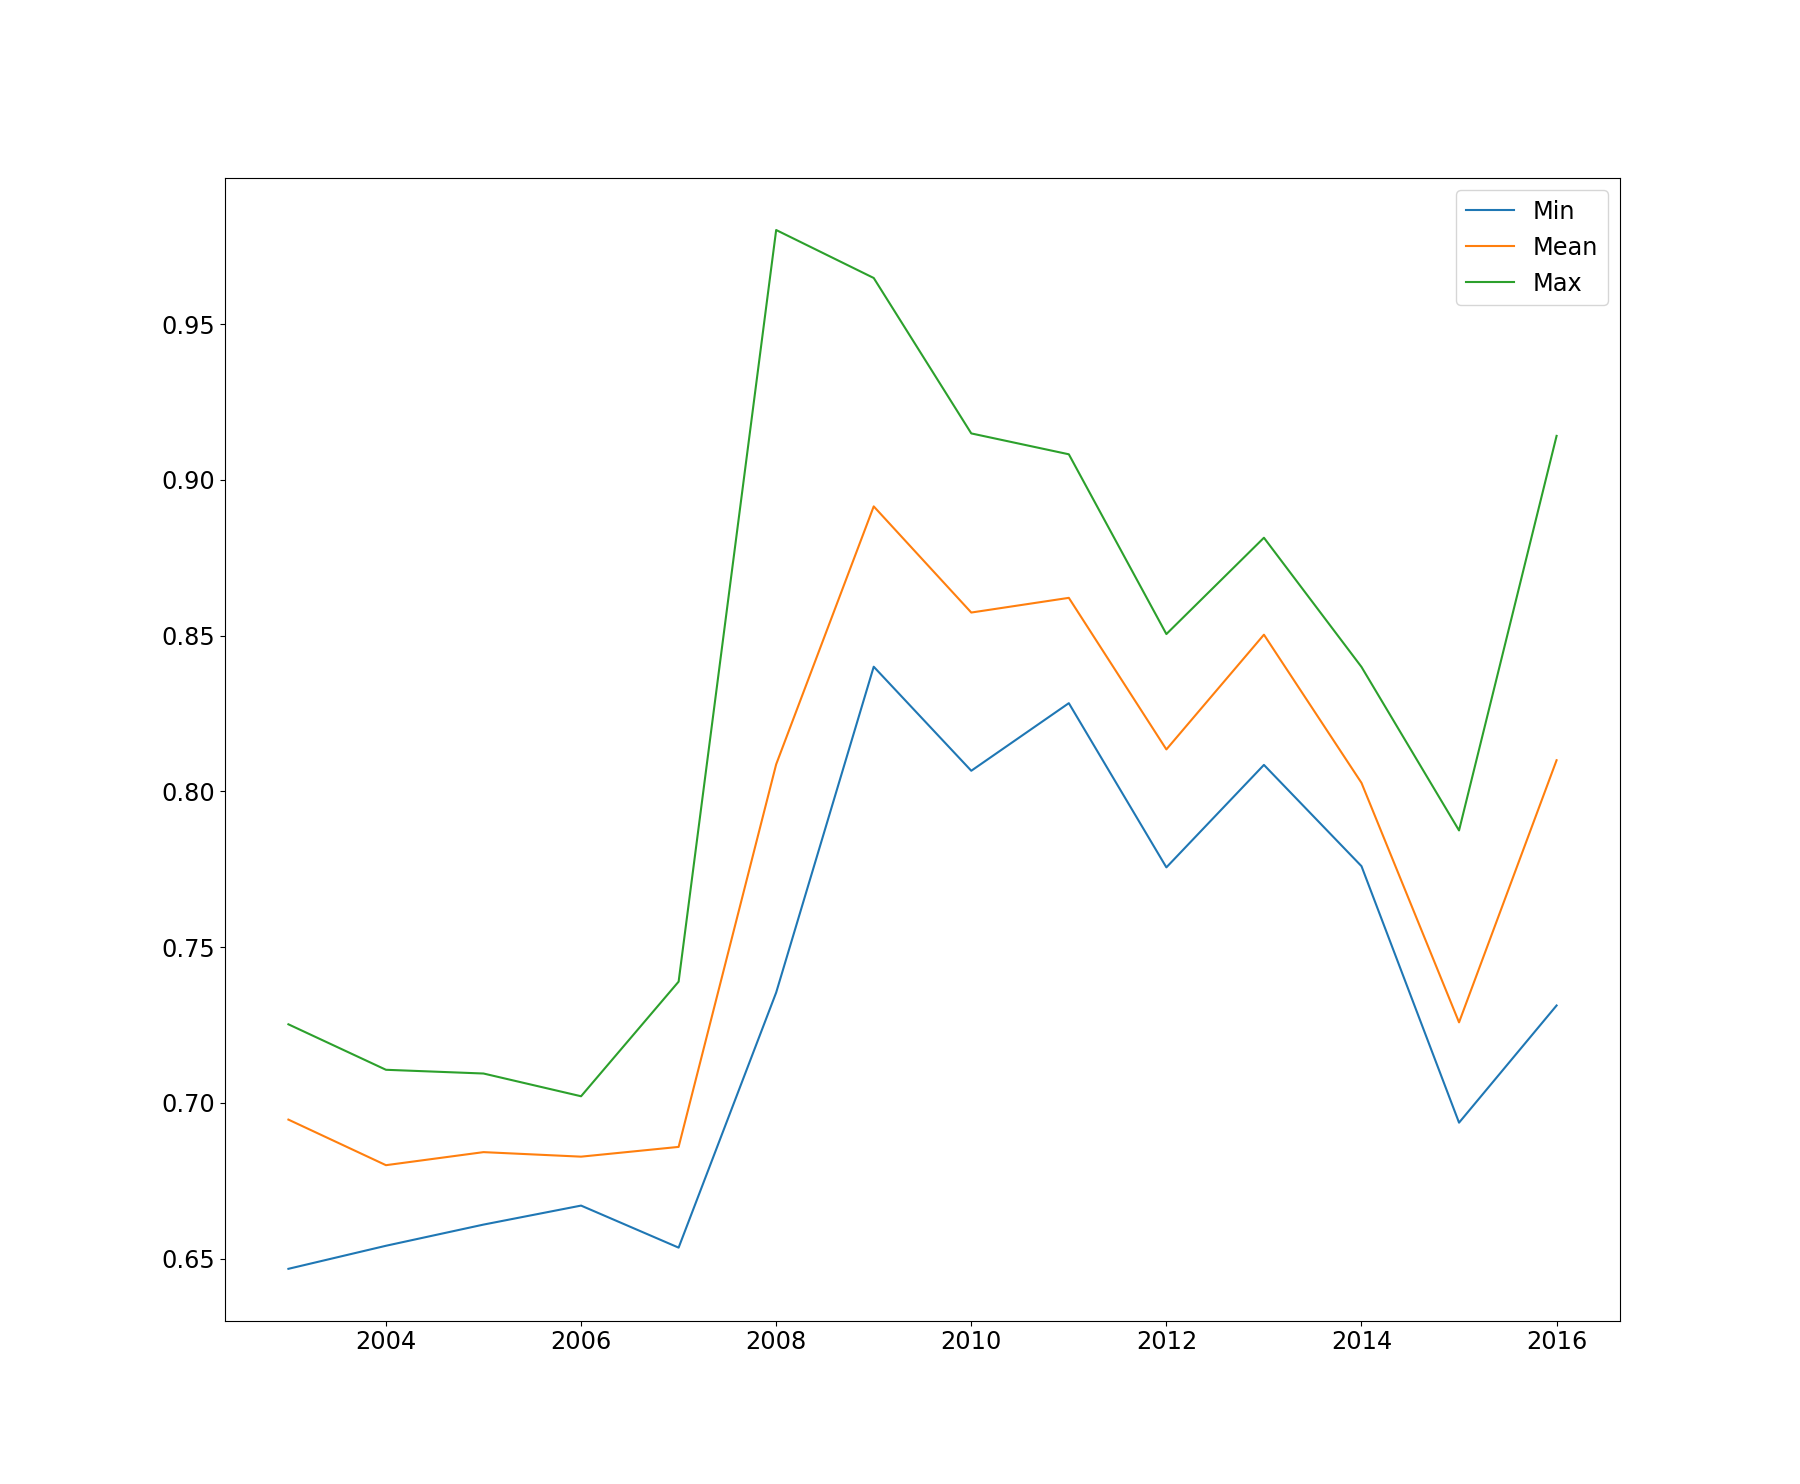
\includegraphics[width=\linewidth]{Figures/stats_gbp}
	\captionof{figure}{Min, Mean and Max of EURGBP each year}
	\label{fig:4}
	\end{minipage}
	\begin{minipage}{.5\textwidth}
	\centering
	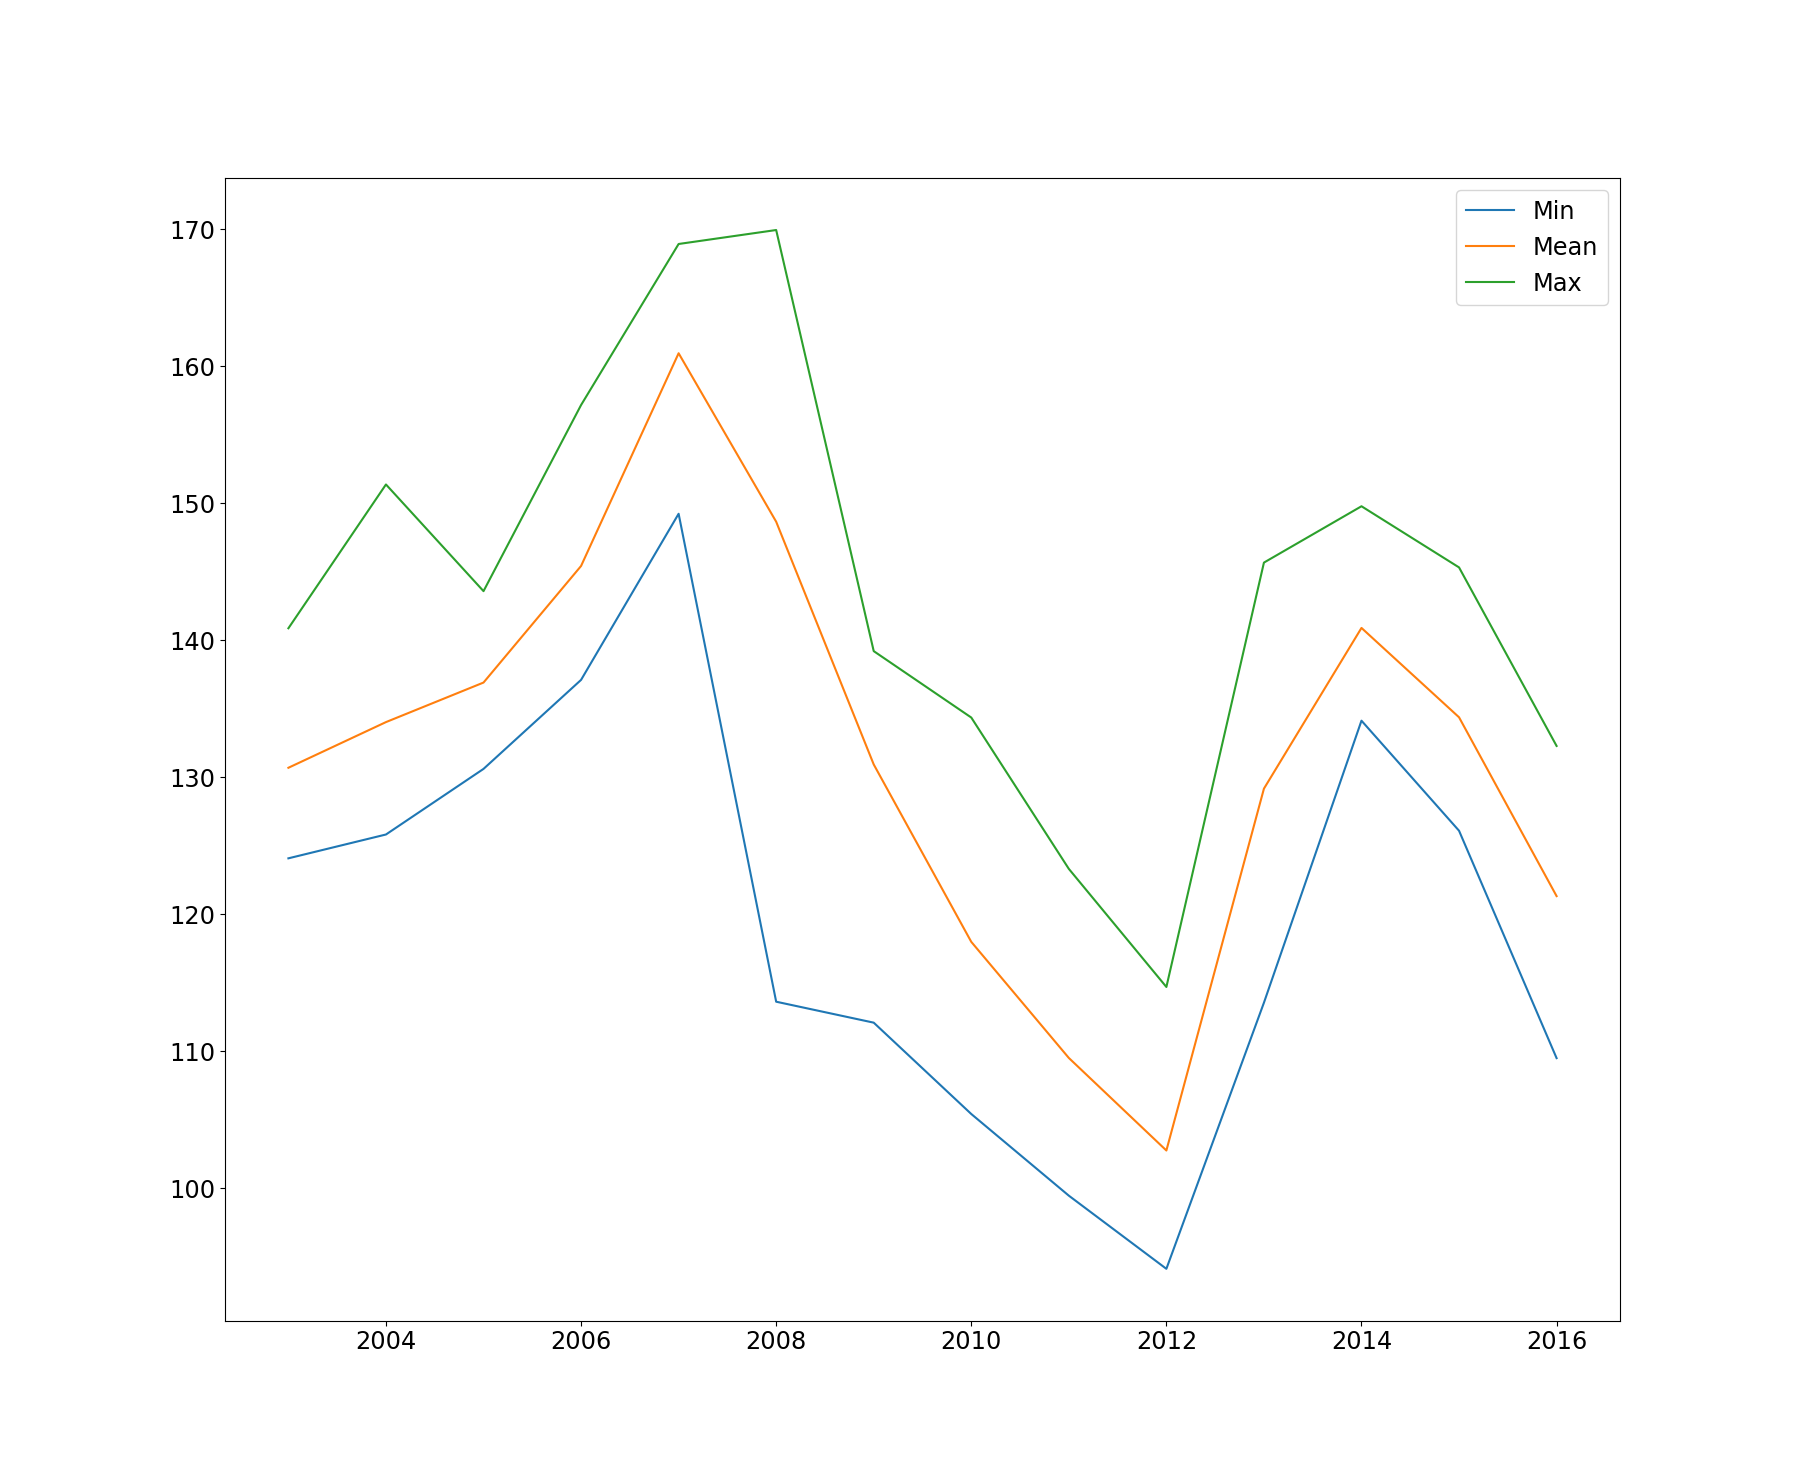
\includegraphics[width=\linewidth]{Figures/stats_jpy}
	\captionof{figure}{Min, Mean and Max of EURJPY each year}
	\label{fig:5}
	\end{minipage}%
	\begin{minipage}{.5\textwidth}
	\centering
	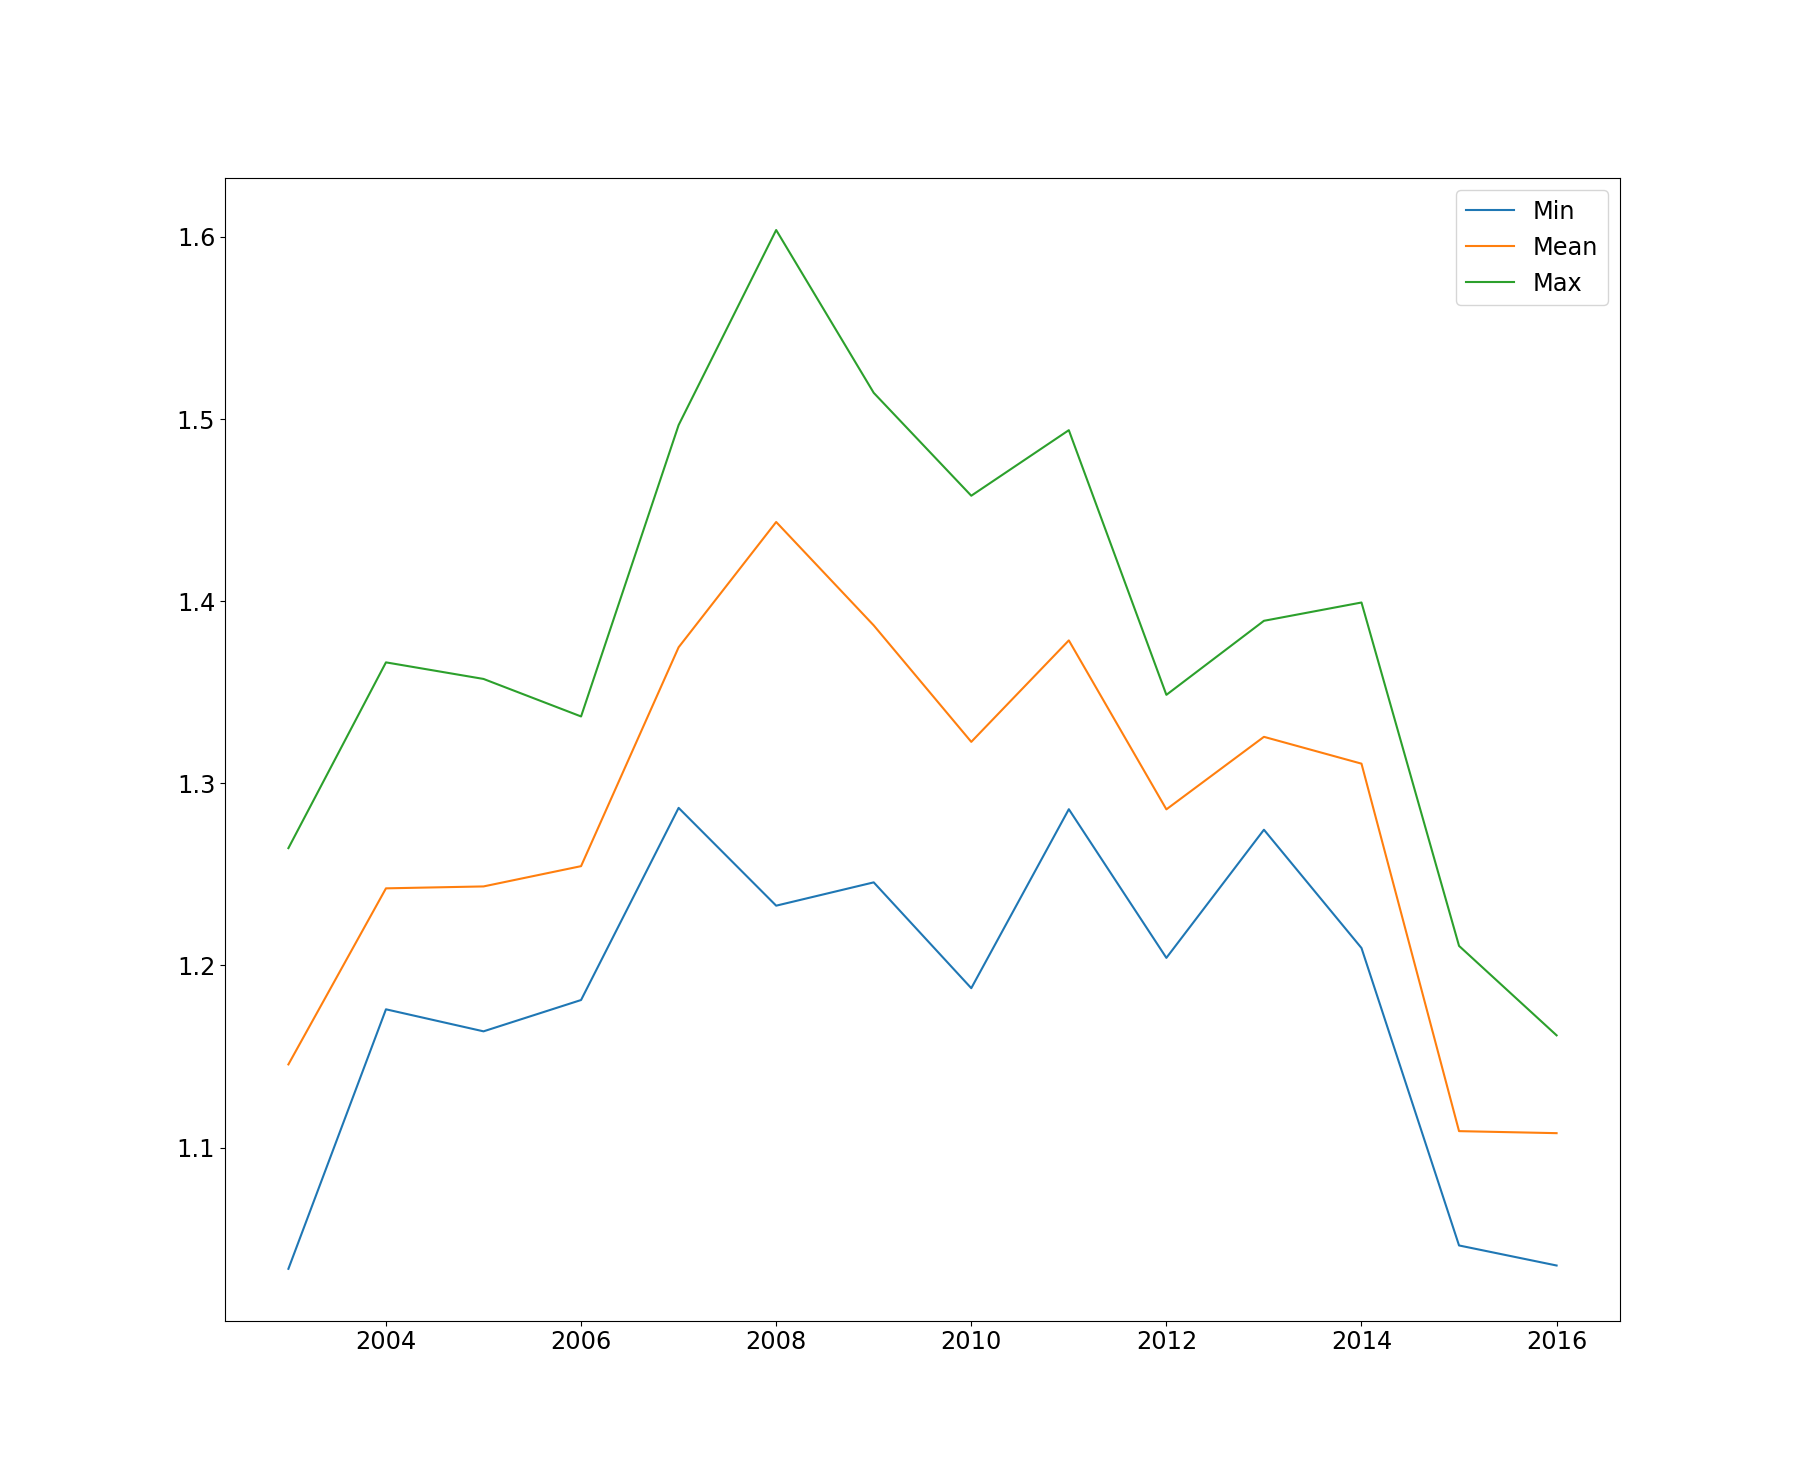
\includegraphics[width=\linewidth]{Figures/stats_usd}
	\captionof{figure}{Min, Mean and Max of EURUSD each year}
	\label{fig:6}
	\end{minipage}
\end{figure}


\section{Mean Reversion Strategy}

The FX environment is famous for its mean reverting properties. We tried to exploit them by developing this strategy. The main idea behind it is that the price process is quite stable and, when a big event happens, the market can overreact and will then return to a more balanced level. Since we are only looking at the price process, our approach is very limited because we must decide whether there was an overshoot just from the magnitude of the shock and this is not trivial.\\
In Figure \ref{fig:7} and \ref{fig:8} we report two extreme cases of what we have just said. In Figure \ref{fig:7} the mean reversion effect is almost not present, the jumps are neat and they are not followed by a recall. In Figure \ref{fig:8}, on the contrary, we have some nice oscillations that we managed to exploit. The two lines that we plotted are the Bid and the Ask.

\begin{figure}[h]
	\centering
	\begin{minipage}{.5\textwidth}
		\centering
		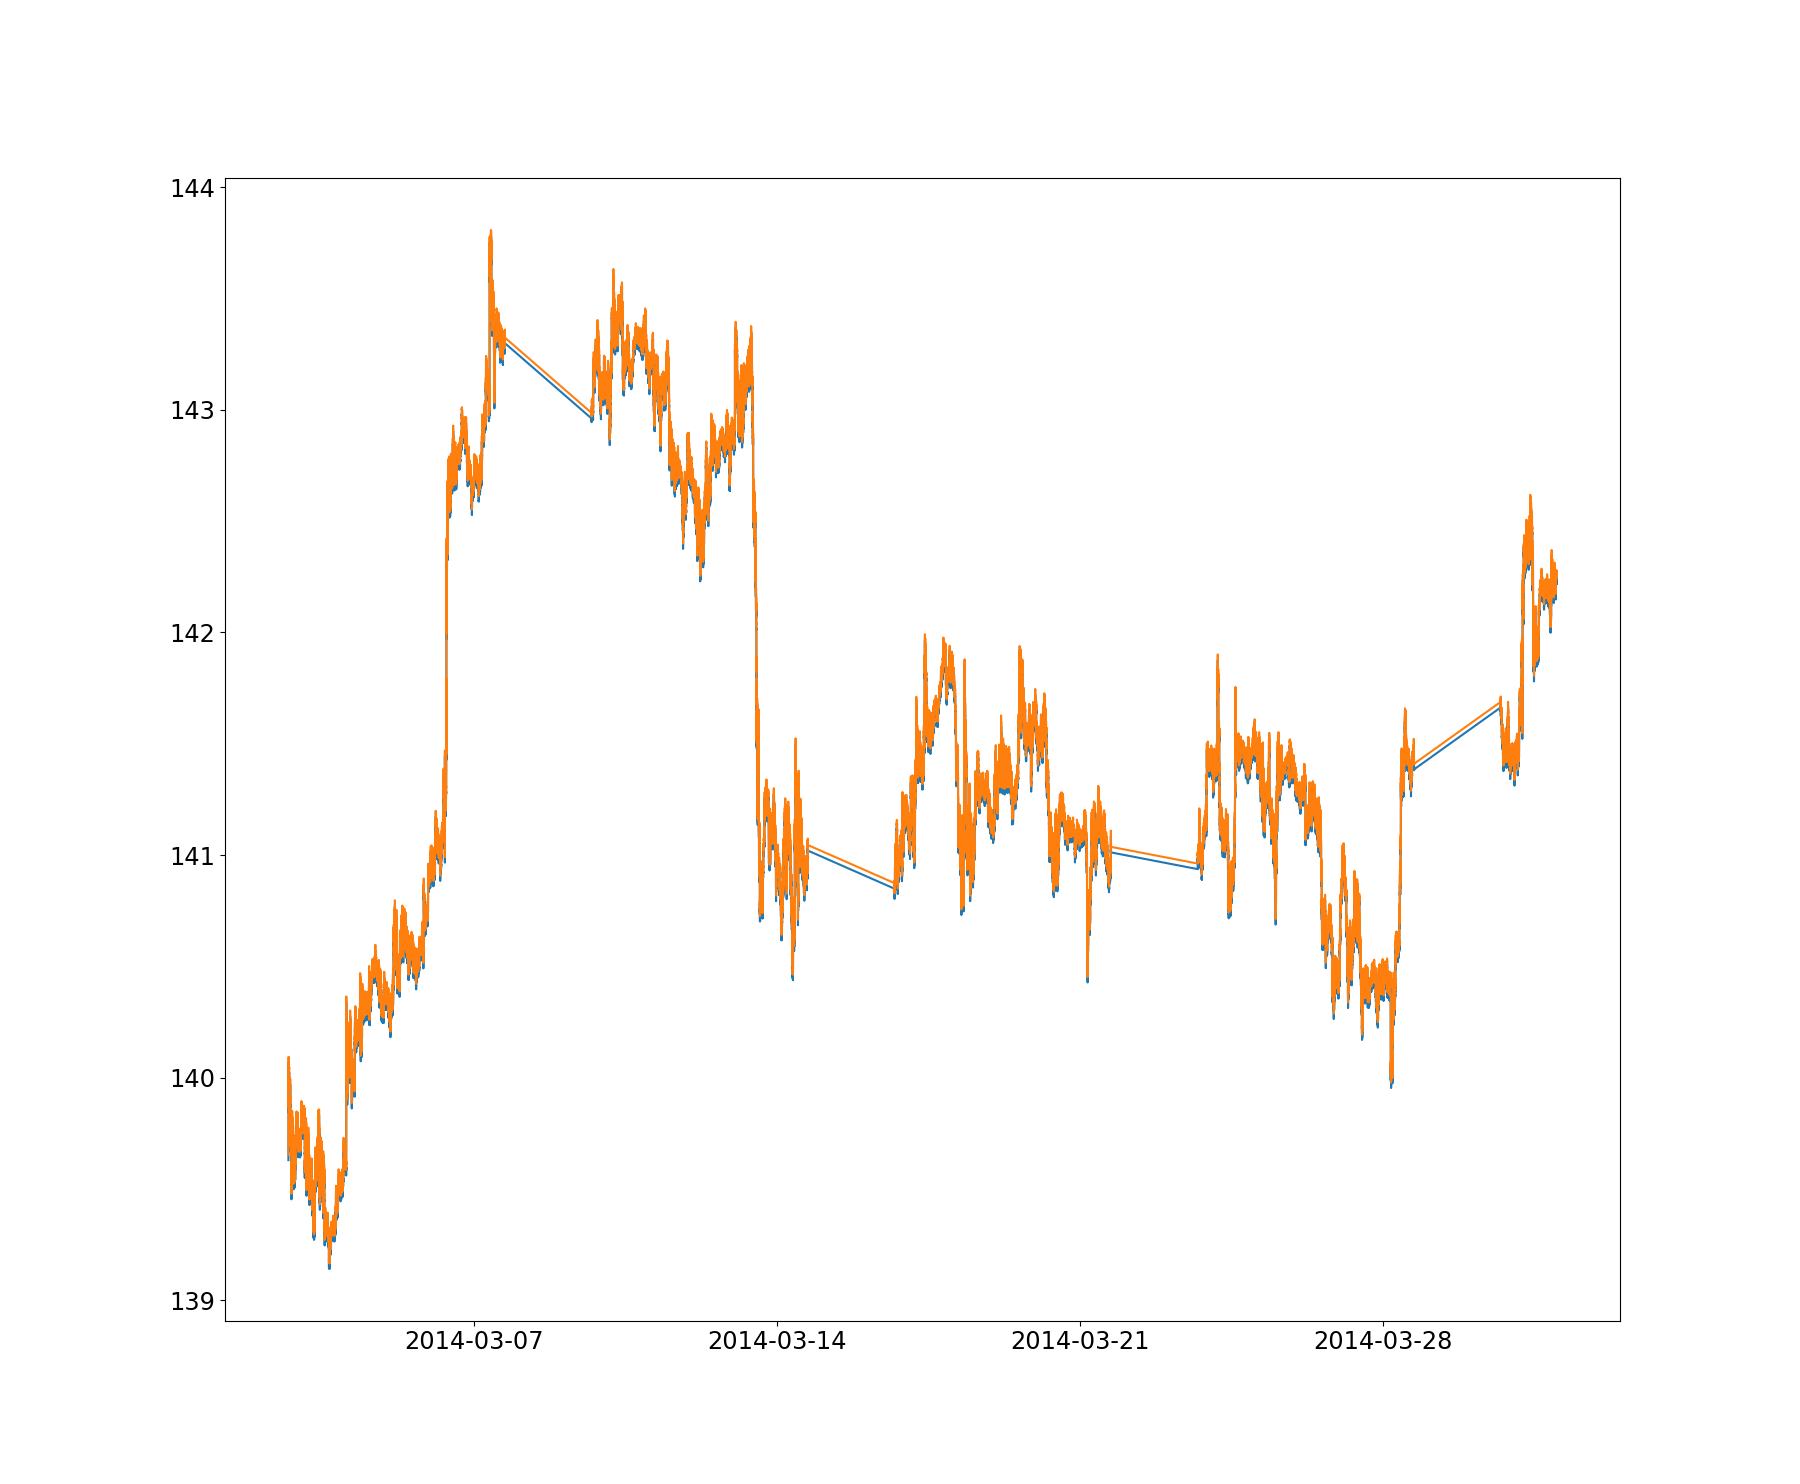
\includegraphics[width=\linewidth]{Figures/strat_1_bad_jpy_14_03}
		\captionof{figure}{EURJPY, March 2014:\\bad month for our strategy}
		\label{fig:7}
	\end{minipage}%
	\begin{minipage}{.5\textwidth}
		\centering
		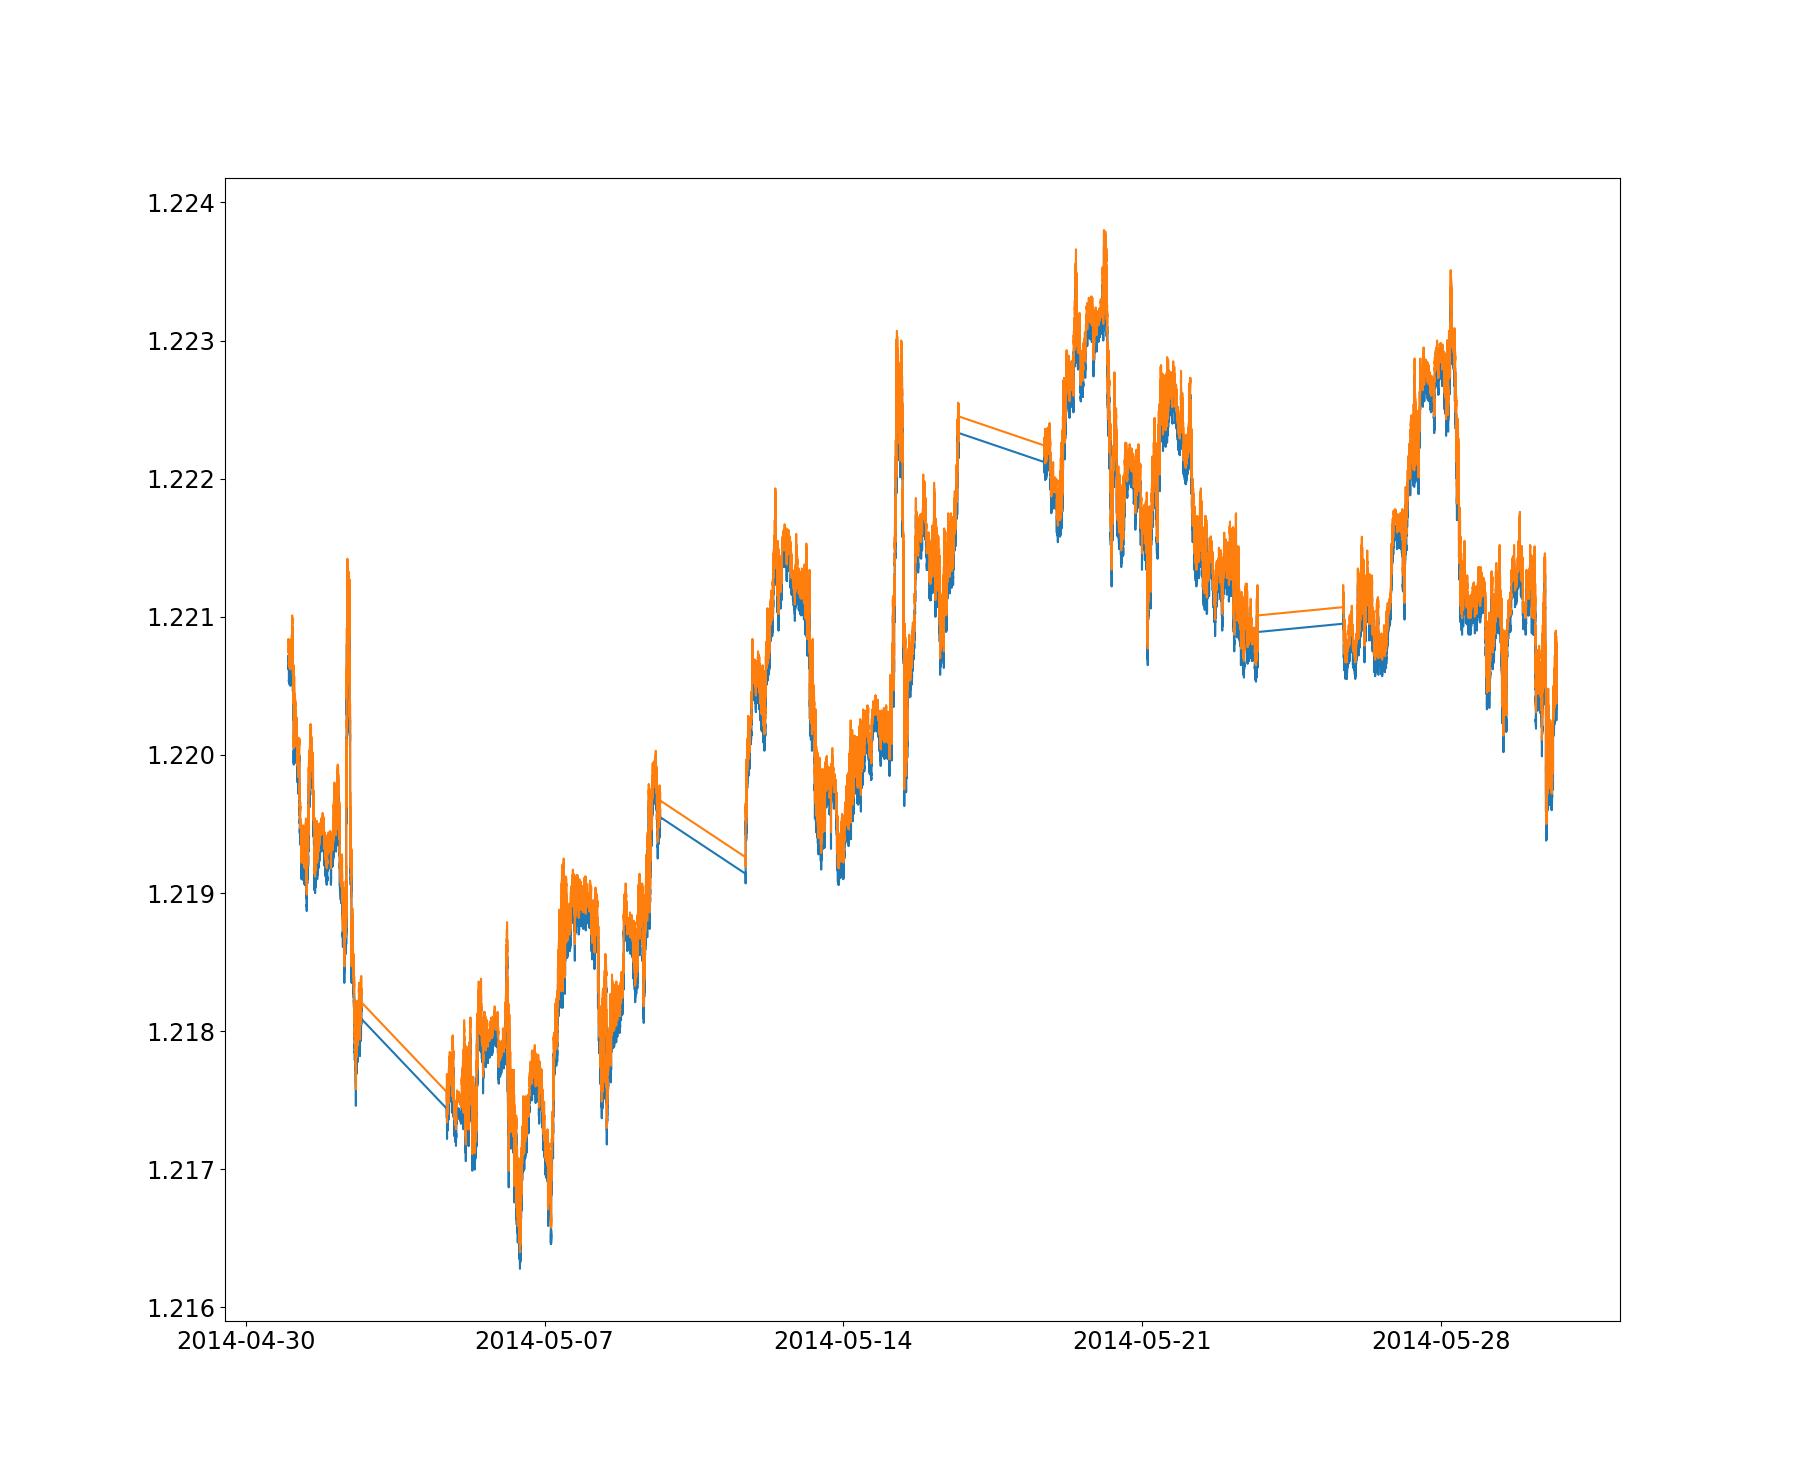
\includegraphics[width=\linewidth]{Figures/strat_1_good_chf_14_05}
		\captionof{figure}{EURCHF, May 2014:\\good month for our strategy}
		\label{fig:8}
	\end{minipage}
\end{figure}

\subsection{Implementation}

As it was said before, the idea behind this strategy is quite simple: when the price goes too high you short, when it goes too low you buy. The difficult part is how to understand if the price was too high or too low.\\
We did that by introducing a long-term mean and a short-term mean. When the difference between the two reached a threshold, we opened a position. We wanted the threshold not to be just a fixed amount, but to reflect the current volatility too. Computing the rolling standard deviation was not possible for our amount of data, so we used the spread as a proxy for it. Finally, the threshold was computed as a hard-coded multiplier times the spread.\\
To summarise, this is the core of our strategy:
\begin{verbatim}
      if (df['short_mean']-df['long_mean'] >  df['spread']*multiplier) ---> SHORT
      if (df['short_mean']-df['long_mean'] < -df['spread']*multiplier) --->  LONG
\end{verbatim}
We fixed the windows for the long-term mean and the short-term mean to 500 and 3, respectively. Once the strategy was triggered, we would hold the position for a fixed amount of data points (80) or until an opposite action was triggered.\\
The multiplier was decided once a year, based on what would have worked the best in December of the year before. We ranked the performance based on the cumulative return. The multiplier could vary between 3 and 20.\\
This strategy was implemented to be able to handle the huge amount of data that we downloaded. In order to do that, we decided to use \emph{Dask}. This limited our possible actions, but the whole process took only 1 hour.

\subsection{Results}

Due to its simplicity and to the clear challenges that we presented above. The performance of this strategy was overall quite terrible. The pair EURJPY in particular was the one where we would have lost money every single year. We suspect that this happened because it is quite typical to find big jumps without recall in this series and this is not compatible with our strategy.\\
Interestingly, the performance, reported in Figure \ref{fig:9}, in the other currency pairs increased in magnitude over the years. It is overall quite negatively skewed, with frequent small gains and some sporadic very big losses (e.g. we can see the effect of Brexit on EURGBP). Since we are calibrating the multiplier only on past data, this could be considered already as an out-of-sample performance, but we had already explored this data so we labelled it as in-sample.\\
We decided to test our strategy out-of-sample for all the currency pairs except EURJPY and we reported the cumulative results in Figure \ref{fig:10}. Here, the training was done monthly on the data of the previous month. We were not surprised to find that their performance was not exceptional in this case too.


\begin{figure}[h]
	\centering
	\begin{minipage}{.5\textwidth}
		\centering
		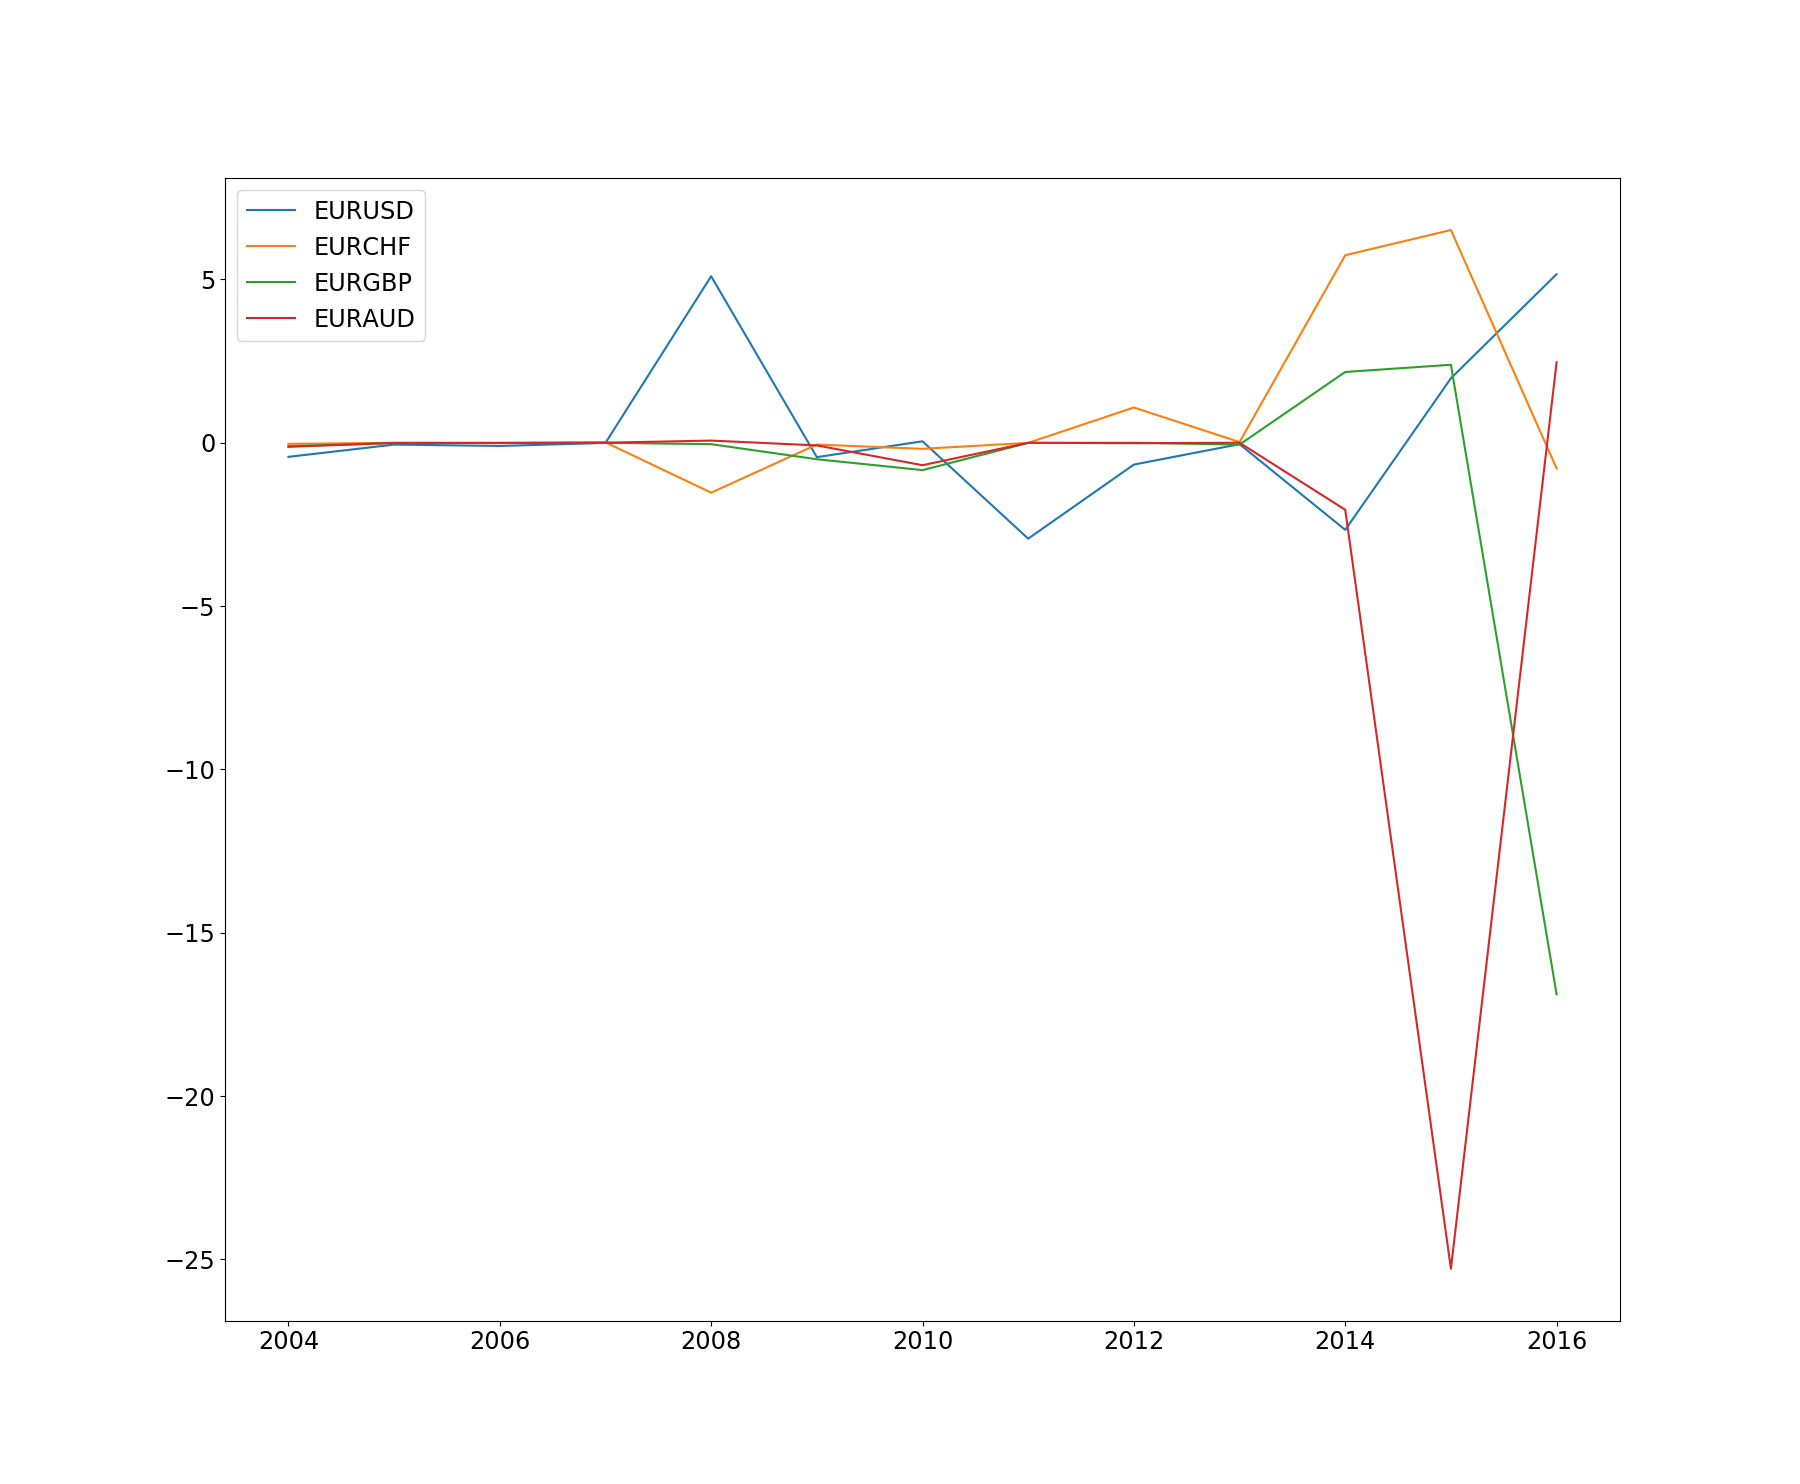
\includegraphics[width=\linewidth]{Figures/strat_1_performance_in}
		\captionof{figure}{Yearly in sample performance}
		\label{fig:9}
	\end{minipage}%
	\begin{minipage}{.5\textwidth}
		\centering
		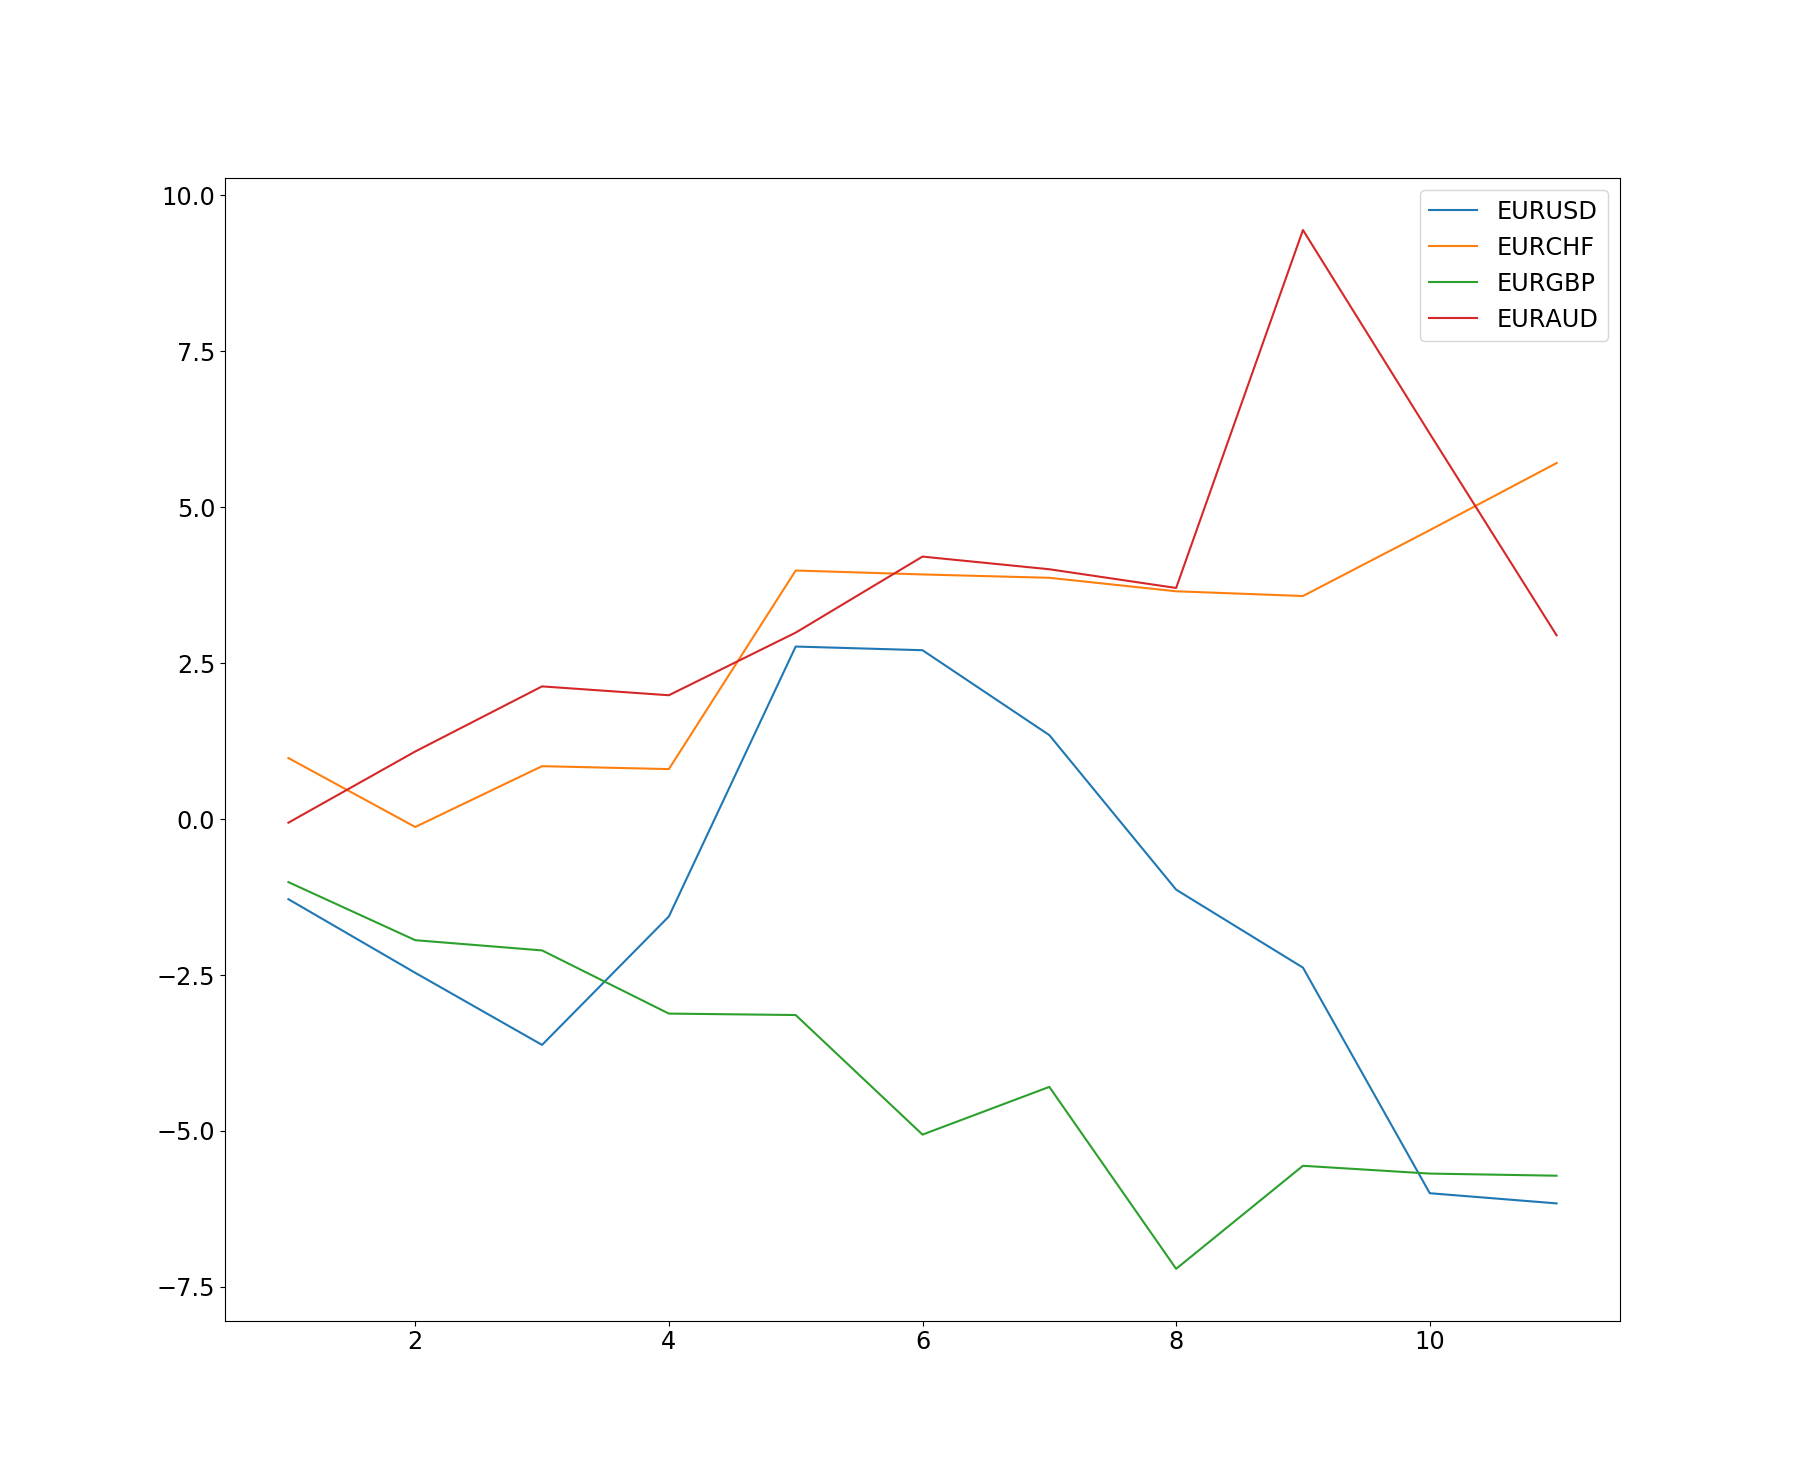
\includegraphics[width=\linewidth]{Figures/strat_1_performance_out}
		\captionof{figure}{Cumulative out of sample performance for 2017}
		\label{fig:10}
	\end{minipage}
\end{figure}

\subsection{Outlook}

There is definitely a lot that can be improved in this strategy. For instance, instead of holding the position for a fixed amount of data entries, we could have implemented two other thresholds: one where we exited if the strategy worked and a stop-loss threshold. However, the training time to find optimal amounts for those thresholds would have been too big.\\
Another big issue is that sometimes we are entering the position too soon and we are not profiting from the whole recall. Handling better the entering time would definitely improve the performance.\\
At the moment, we are only tuning the value of the multiplier. To choose the other parameters we compared the performance of the strategy in the first months of 2003. If they were allowed to evolve, there could be an improvement.\\
Finally, a mean reversion strategy essentially implies trading on noise and hoping that it will be reabsorbed. Currently, we are approximating the trend as the long-term mean and the noise as the difference between that and the short-term mean. This is clearly not the best approximation and, being at the heart of our model, it affects greatly its performance. We did it in this way because we were focusing our attention in developing a strategy that was computationally very efficient and able to crunch 14 years of tick-by-tick data in an hour. A smarter algorithm would have probably achieved a better performance at the expense of the computational time.







\end{document}
